%%==========================================================================
\section{Experiments}
\label{sec:experiments}

We have used synthetically generated data as well as real captured data to evaluate the SuperMatching algorithm.
To demonstrate the independence and generalization of the SuperMatching, different descriptors have been applied.
For 2D deformable surface, SIFT~\cite{Lowe04} are used.
While for the 3D shapes without color information, slippage features~\cite{Bokeloh08} are employed.
For 3D colorful shapes, both SIFT and slippage features are employed.
To build the matching between two shapes, we used third-order matching for the experiments.
For greater than third higher-order, it is easy to replace the potential by relevant polygonal definitions.

%-------------------------------------------------------------------------
\subsection{2D deformable surfaces}
\label{subsec:2DDeformable}

Firstly, we used a 2D deformable surface data \footnote{From \url{http://cvlab.epfl.ch/data/dsr/}} with a cloth and a cushion.
The surfaces of the cloth underwent relatively smooth deformations, while the surfaces of the cushion included sharp folds.
The data has provided ground truth, which are very useful to verify the accuracy quantitatively.
From each image set we randomly chose six frames before and after a large deformation.
We randomly chose $100$ corresponding points on each surface to be the features, using the provided ground truth.
In each image set we chose the features on the frame most unlike the others as $P_1$ and matched them with the features in the other five frames.

We used the data as a basis for comparison with the spectral algorithm~\cite{Cour06} (a quadric assignment algorithm),
a third-order tensor algorithm~\cite{Duchenne09},
and the hyper graph matching algorithm~\cite{Zass08}, using the authors' code in each case.
All methods were executed in Matlab on a $2.3$GHz Core2Duo with $2$GB memory.
To enable direct and fair comparison,
~\cite{Duchenne09}, ~\cite{Zass08} and SuperMatching used the same potential and all maintained an equivalent tensor size.

In the tests, SuperMatching used $20000$ feature tuples, while the method of~\cite{Duchenne09} used 1010000 features  and the method of~\cite{Zass08} used $40000$.
The difference is mainly resulting from the effects of sampling strategy, and it could prove that our sampling is effective to reduce the sampling cost.
The average running time to match two feature sets each with $100$ features was around 8s for SuperMatching, 13s for~\cite{Duchenne09}, 6.5s for~\cite{Zass08}, and $5$s for~\cite{Cour06}.
So, as we use same tensor size but fewer feature tuples, SuperMatching is performed with less computation than third-order tensor algorithm~\cite{Duchenne09}.

The matching accuracy is given as the number of correctly matched points (according to the provided ground truth) divided by the total number of points that could potentially be matched.
The results for all algorithms, using the two image sets, are given in Table~\ref{tab:errorrate1} and are illustrated in Figure\ref{fig:2DDeformable}.
Table~\ref{tab:errorrate1} demonstrates that we achieve a higher matching accuracy than previous algorithms.
The worsest matching result is produced by the spectral quadratic assignment algorithm~\cite{Cour06},
due to the powerless solution from the pairwise geometric constraints.
The results also show that higher-order algorithms perform much better due to the more complex geometric constraints.
However, the third-order algorithm~\cite{Duchenne09} and the hyper graph matching algorithm~\cite{Zass08} do not perform well,
because the geometric relationships among elements are not established accurately from the supersymmetric tensor.

%----------------------------------------
%  deformable matching results IMAGES
%----------------------------------------
\begin{figure}
\centering
  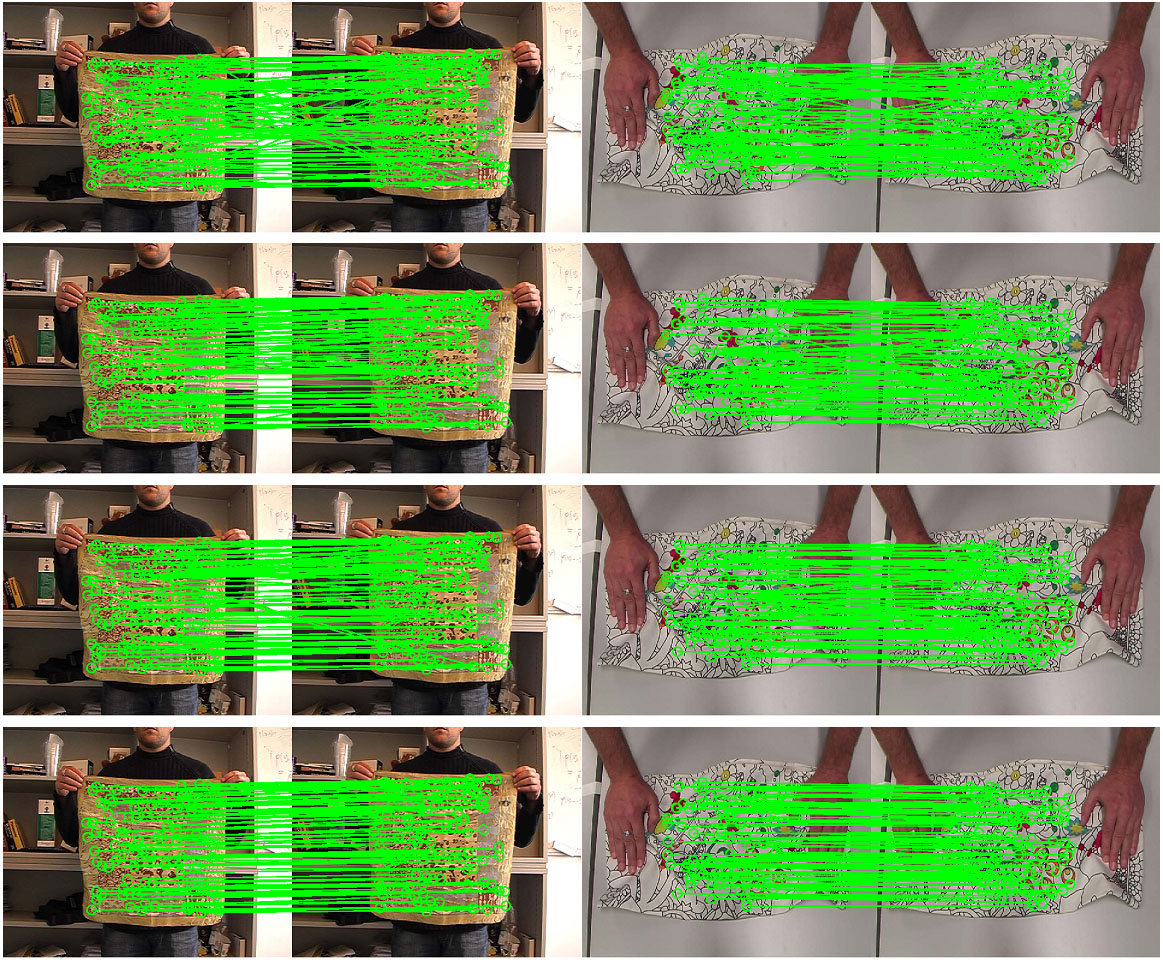
\includegraphics[width=1.00\linewidth]{figures/2DDeformable.jpg}
  \caption{Matching results. Left: cloth set, selected from frame 85 to 110, right: cushion set, selected from frames 144 to 213.
  Top to bottom, spectral method [Cour et al. 2006], hyper graph matching method [Zass and Shashua 2008], a Third-order tensor [Duchenne et al. 2009], and our SuperMatching algorithm.}
\label{fig:2DDeformable}
\end{figure}

%----------------------------------------
%  deformable matching results TABLE
%----------------------------------------
\begin{table}
%\vspace{-4mm}
\centering
%\renewcommand{\arraystretch}{0.8}
\tabcolsep=1pt
\setlength{\aboverulesep}{0pt}
\setlength{\belowrulesep}{0pt}
\caption{Error rate of deformable surface matching.}
\hspace{-5ex}
\label{tab:errorrate1}
\small
\begin{tabular}{l|c c c c | c c c c | c c}
\toprule
{Dataset}  & \multicolumn{4}{|c|}{ {cloth}} & \multicolumn{4}{c|}{ {cushion}} & & \\
\hline
 {Matching frames} &  {F80-}	&  {F90-}	& {F95-}	& {F100-} & {F144-} & {F156-}	& {F165-}	& {F172-} & {Feature}	& {Time}  \\
 {}                &  {F90 }    &  {F95 }   & {F100}    & {F105}  & {F156}  & {F165}    & {F172}    & {F188}  & {Tuples}    &  {(s)} \\
\hline
 {SuperMatching}   &  {17\%}    &  {15\%}	& {16\%} 	& {19\%}  & {34\%}	& {40\%}	& {31\%}	& {44\%}  &  {20k}	    &  {8}  \\
%\hline
 {\cite{Zass08}}   & {27\%}	    & {21\%}	& {30\%}	& {28\%}  & {56\%}  & {61\%}    & {46\%}	& {57\%}   & {40k}	    & {6.5}  \\
%\hline
{\cite{Duchenne09}} & {33\%}    & {23\%}    & {27\%}	& {35\%}  & {61\%}	& {69\%}	& {53\%}	& {58\%}   & {1010k}    & {13}  \\
%\hline
 {\cite{Cour06}}   & {73\%}     & {71\%}	&  {78\%}	& {73\%}  & {86\%}  & {95\%}	& {72\%}	& {93\%}   & {--}       & {5}  \\
\bottomrule
\end{tabular}%
%\vspace{-27pt}
%\vspace{-8mm}
\end{table}%
%

%-------------------------------------------------------------------------
\subsection{3D rigid shape scans}
\label{subsec:3DRigid}

Secondly, we used the SuperMatching to alignment multiple 3D rigid shape scans.
For the multiple scans, the Third-order matching is first performed between two consecutive frames.
Then rigid transforms can be computed from the three compatible matching feature points.
The transform which brings the most data points within a threshold of a point in the model is chosen as the optimal aligning transform~\cite{Huttenlocher90}.
As stated by~\cite{Gelfand05}, the voting scheme is guaranteed to find the optimal alignment 
between the pairwise scans and is independent of the initial pose of the input scans.
After the initial pairwise matching, the alignment is refined by the iterative closest point (ICP) algorithm similar to~\cite{Gelfand05}.
Figure~\ref{fig:3DRigid} demonstrates the former explains.
On the up, the sheep head object is captured from different viewpoints, and relevant scans are generated.
Relative position and orientation of 10 scans is then be computed to produce a single merged shape.
The linkage segments between consecutive scans imply where the SuperMatching algorithm is applied.

\begin{figure}
\centering
  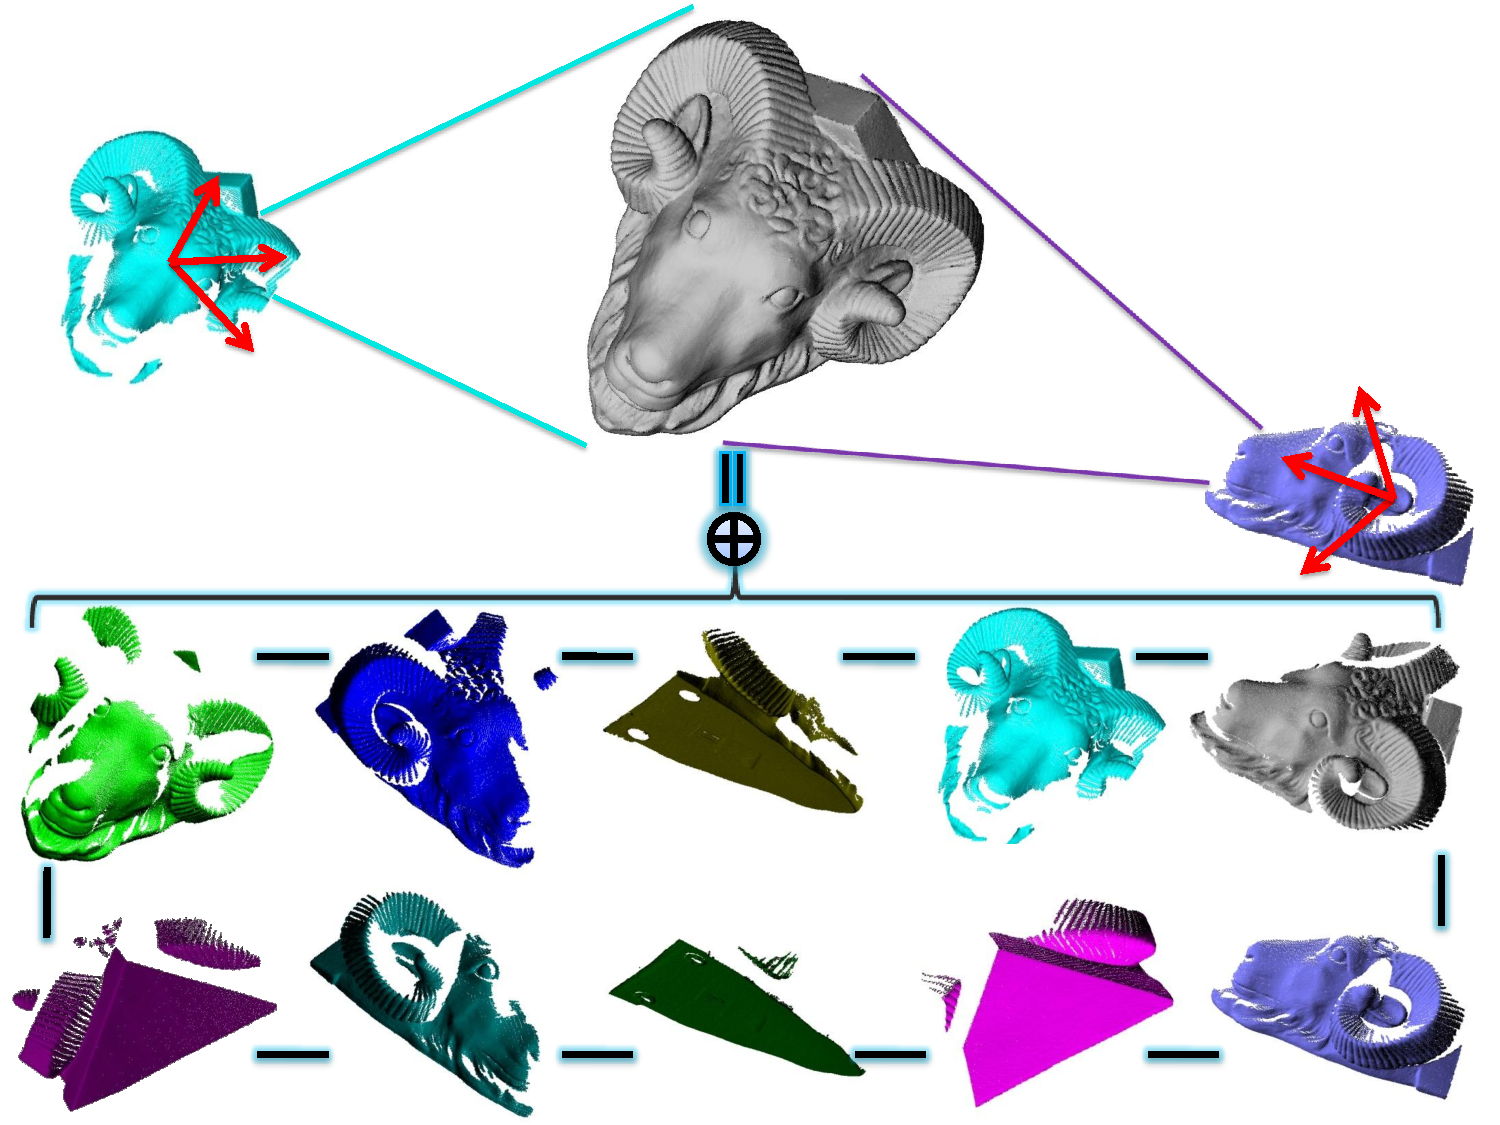
\includegraphics[width=0.99\linewidth]{figures/3DRigid.pdf}
  \caption{The alignment of rigid sheep head scans. The scans are captured from different viewpoints (up), and the final aligned shape is formed from 10 scans (bottom).}
\label{fig:3DRigid}
\end{figure}

%-------------------------------------------------------------------------
\subsection{3D articulated shape synthetic data}
\label{subsec:3darticulated}

Thirdly, we present another application, articulated registration, to address these challenges by reconstructing an articulated 3D shape from dynamic range scans. 
Given a sequence of range scans of a moving articulated subject, the method automatically registers all data to produce a complete 3D shape.
The advantages of the method is that it does not require any manual segmentation, user specified markers, nor a prior template.
Ultimately, the problem of non-rigid registration of deformable shapes is ill-posed and no algorithm is applicable to all scenarios. 
We believe, however, that our approach pushes the limits of what can be achieved with minimal prior information, and is robust to the partial data with holes.

The articulated registration is performed in two main steps. 
We first precomputing an initial pairwise registration for each pair of consecutive frames, then the articulated shape reconstruction similar as~\cite{Pekelny08}.
Although the partial scans have missing data and their poses are different, the SuperMatching could produce accurate matching.
Using the correspondences established by the SuperMatching, the robust registration of scans are obtained by computing the piecewise rigid transformations.
Then, we propagate the transformations assigned from the slippage feature points subset to all points using nearest neighbor interpolation.
The incidental outcomes of pairwise registration include the rigid parts detection by clustering the transformation and segmenting the partial data.
The transformation clustering is done by mean shift algorithm~\cite{Comaniciu02}, which is a robust non-parametric method based on gradient ascent.
Therefore, after the initial pairwise registration, the consecutive two partial data has been registered and each data has been segmented according to the transformation. 
The outcome would be used as the input for the second step articulated shape reconstruction~\cite{Pekelny08}.
The algorithm identifies and tracks the rigid parts in each frame, while accumulating the geometric information over time.
For more details on articulated shape reconstruction with segmentation information, we refer to~\cite{Pekelny08}.

Although our method is partly taking the technique from the articulated motion capture and reconstruction method~\cite{Pekelny08}. 
However, ~\cite{Pekelny08} requires the user to manually segment a range scan in advance, 
whereas we automatically solve for the segmentation using the transformation computed in all frames by the initial pairwise registration.

Figure~\ref{fig:3DHand} shows one articulated hand example.
The partial synthetic data is generated from deformation sequence, and the final registered shape is produced from these partial data.
We also evaluate the robustness of our reconstruction method using the ground truth, comparison shown in Figure~\ref{fig:3DHand} center.
Quantitatively, we measured the maximum of the average distance over all frames as 0.001, 
the maximum of the maximum distance over all frames as 0.012 as a fraction of the bounding box diagonal.

\begin{figure}
\centering
  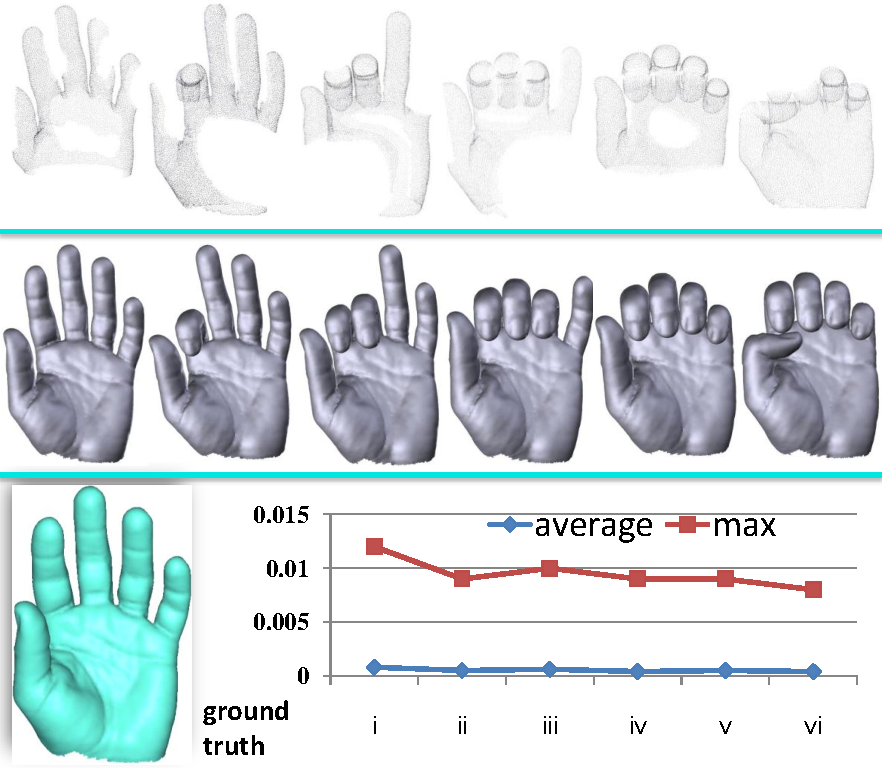
\includegraphics[width=0.99\linewidth]{figures/3DHand.pdf}
  \caption{The registration of articulated hand. 
  The partial synthetic data (up) is generated from deformation sequence, and the reconstructed shapes recover the motion (center).
  The reconstructed shapes are compared with relevant ground truth (bottom), 
  the graph shows the maximum and average error distance between the ground truth and the reconstruction for each frame.}
\label{fig:3DHand}
\end{figure}

%-------------------------------------------------------------------------
\subsection{3D colorful real depth scans}
\label{subsec:3dColored}

Complementary to the extensive evaluation presented above, 
we also provide a real-world example demonstrating matching using the SuperMatching. 
Figure~\ref{fig:3DReal} shows a matching result from exhibiting various transformations of KINECT camera~\cite{Kinect12}. 
The matching with both SIFT and slippage features was performed by the SuperMatching,
resulting in robust matches without significant outliers.

\begin{figure}
\centering
  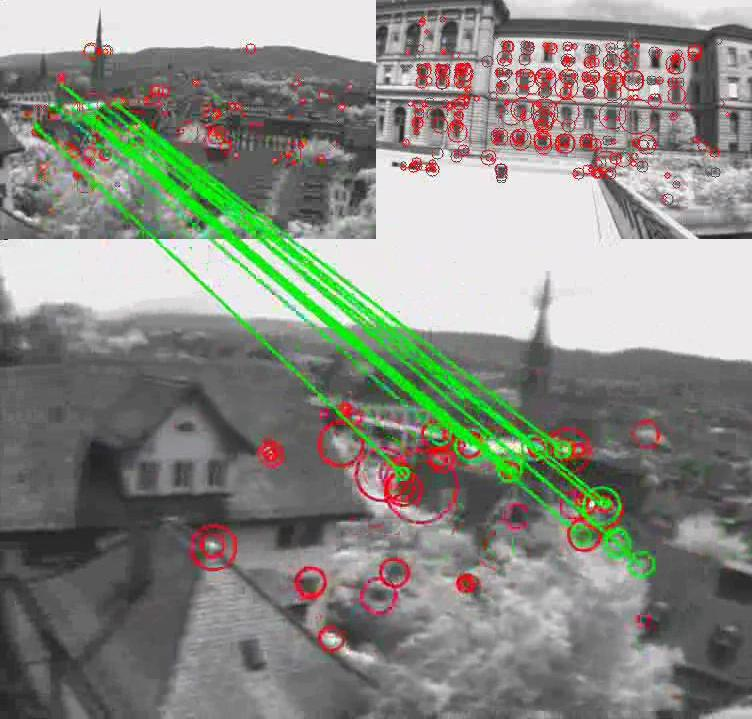
\includegraphics[width=0.98\linewidth]{figures/3DReal.jpg}
  \caption{3D colorful real depth scans from KINECT. 
  Two given different local pre-scans are shown on the up. The real varying depth data is captured by KINECT, and one snap is listed on the bottom. 
  The matching points are connected by the green lines.}
\label{fig:3DReal}
\end{figure}
